\chapter{角动量理论}
%%%%%%%%%%%%%%%%%%%%%%%%%%%%%%%%%%%%%%%%%%%%%%%%%%%
%%%%%%%%%%%%%%%%%%%%%%%%%%%%%%%%%%%%%%%%%%%%%%%%%%%

\section{角动量}
%%%%%%%%%%%%%%%%%%%%%%%%%%%%%%%%%%%%%%%%%%%%%%%%%%%
\paragraph*{角动量算符} 角动量算符满足的的充要条件如下
\begin{theorem}{角动量算符的充要条件}
	\begin{equation}
		J^{\dagger}_k = J_k, ~ k = 1, 2, 3, \quad \left[J_i, J_j\right] = i\hbar \sum_{k} \epsilon_{ijk} J_k
	\end{equation}
\end{theorem}
其中,$\epsilon_{ijk}$是反对称的三维Levi-Civita排序符号。其有如下性质:1. 若有两个指标相同,则$\epsilon_{ijk} = 0$;2. 若三个指标两两不等,按循环排序,即如下图所示的排序时,有$\epsilon_{123} = \epsilon_{231} = \epsilon_{312} = 0$;3. 剩下的排序将使排序符号为$-1$。
\begin{figure}[htbp]
	\centering
	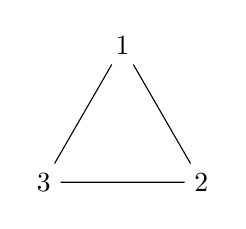
\begin{tikzpicture}
		\node (A) at (0,0) {3};
		\node (B) at (2,0) {2};
		\node (C) at (60:2) {1};
		\draw (A) -- (B) -- (C) -- (A);
	\end{tikzpicture}
\end{figure}

\paragraph*{角动量算符的本征态和本征值} 角动量$\boldsymbol{J}$的本征态和本征值如下
\begin{align}
	\boldsymbol{J}^2 |j\ m\rangle =& j(j+1)\hbar^2 |j\ m\rangle	\\
	J_z |j\ m\rangle =& m\hbar |j\ m\rangle
\end{align}
其正交性和归一性为
\begin{equation}
	\langle j^{\prime}\ m^{\prime} | j\ m\rangle = \delta_{jj^{\prime}}\delta_{mm^{\prime}}, \quad m = -j,\ -j+1, \ \cdots, j-1,\ j \ .
\end{equation}
此外,我们定义角动量的梯度算符
\begin{equation}
	J_{\pm} = J_{x} \pm i J_{y}
\end{equation}
满足对易式
\begin{equation}
	\left[J_{+}, J_{-}\right] = 2\hbar J_z, \quad \left[J_{\pm}, J_{z}\right] = \mp \hbar J_{\pm}
\end{equation}
梯度算符作用到本征态上的效果为
\begin{equation}
	\begin{aligned}
		J_{\pm} |j\ m\rangle =& \hbar \sqrt{j(j+1) - m(m\pm)1} |j\ m\pm 1\rangle	\\
						   =& \hbar \sqrt{(j\pm m +1) (j\mp m)} |j\ m\pm 1\rangle
	\end{aligned}
\end{equation}
对于单粒子在希尔伯特空间中的抽象角动量本征态$|j\ m\rangle$的坐标表示通常为\underline{球谐函数}。

\paragraph*{角动量}

%%%%%%%%%%%%%%%%%%%%%%%%%%%%%%%%%%%%%%%%%%%%%%%%%%%
%%%%%%%%%%%%%%%%%%%%%%%%%%%%%%%%%%%%%%%%%%%%%%%%%%%
\section{角动量耦合}


%%%%%%%%%%%%%%%%%%%%%%%%%%%%%%%%%%%%%%%%%%%%%%%%%%%
\subsection{自旋-轨道耦合}
	自旋轨道耦合

%%%%%%%%%%%%%%%%%%%%%%%%%%%%%%%%%%%%%%%%%%%%%%%%%%%
\subsection{两角动量耦合}
考虑两个完全对易的角动量$\boldsymbol{J}_1$和$\boldsymbol{J}_2$,也就是说这两个角动量分别属于两个不同的粒子,或者是一个粒子的自旋角动量和轨道角动量。


%%%%%%%%%%%%%%%%%%%%%%%%%%%%%%%%%%%%%%%%%%%%%%%%%%%
\subsection{Clebsch-Gordan系数和3-j符号}



%%%%%%%%%%%%%%%%%%%%%%%%%%%%%%%%%%%%%%%%%%%%%%%%%%%
